%
\section{Sorting algorithms}

All of us know that washing black and white together is a bad idea; however there are a lot of criteria to distinguish and prepare clothes for washing. This chapter presents several sorting algorithms for preparation to wash. 

\subsection{Requirements/criteria}

Mostly all of the clothes have the sewed label (tag). There are defined information about fabric, washing temperature and etc. For instance fabric defines the material of clothe –how clothe is sensitive.  For instance wool is more sensitive when synthetic or clothe which can be washed 40 degree is more sensitive than clothe which can be washed 95 degree. Of course sometimes 40 degree clothe can be washed on 30 or 60 degree and 95 degree can be washed on 60 degree temperature. \\ \\ A general criterion’s used to create sorting algorithm:

\begin{itemize}
	\item Colour – often there are bad idea wash white and black together, so this criteria defines that clothes of colored and white should be distinguished and washed separately. 
	\item Washing temperature – some clothes are more sensitive than other, so clothe should be washed on temperature defined by label in other case there could be possibility to damage clothe.
	\item Fabric – defines material of the clothes. For instance wool, cotton, synthetic and etc. All those material types have different sensitive criterions. Comparing wool and synthetic of the same color and temperature we should take in to account that wool is higher priority clothe and same synthetic clothe should be washed regarding rules of wool.
	\item Weight – defines bin size of washing machine size. In other words how many clothes can fit to washing machine and be washed.
\end{itemize}

\noindent Abstract criterion defines how clothes can be washed:

\begin{itemize}
	\item White and light clothes can be washed together
	\item Colored and dark clothes can be washed together
	\item Light, white and cotton often are washed on higher temperatures 60 degree or higher
	\item Cotton and wool can be washed together, however all rules set regarding wool
	\item Daily clothes temperatures around 60 degree
	\item Work clothes temperatures around 90 degree
	\item Washing temperature of wool is low (below 40 degree)
	\item Cotton more sensitive than synthetic
	\item Wool more sensitive than cotton
\end{itemize}

\subsection{Sorting algorithm designs}

\subsubsection{Sorting by color and temperature}

Algorithm presented in figure 8.1 is one of the simplest, which is also implemented. When list of clothes comes to sort, then each clothe are moved to particular bin. First are sorted by color and then by temperature. Number of total possible bins is ten – five for colored and five for white. Bins are numbered automatically.

\begin{figure}[h]
	\centering
		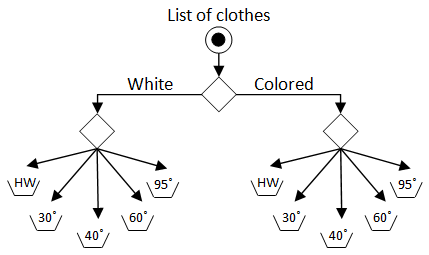
\includegraphics{sortingByColorTemp}
	\caption{Sorting algorithm by color and temperature}
	\label{fig:planning}
\end{figure}

This kind of algorithm is not optimal, because one clothe can be washed as well. Of course if time is not so important, then clothes from the bin should be washed when bin is full.

\subsubsection{Sorting algorithm using configurable parameters}

A lot of laundry institution sorting clothes similar but not the same. One of them has different size washing machines others wash at the higher temperature and all of them have distinct criteria’s.   So question is: how can be created software which satisfied all user requirements. \\  Here presented software based on C\# language, software consists of two parts: configuration and sorting algorithm. Configuration part is finished, however sorting algorithm do not finished. Purpose of the configuration is to save and load sorting criteria’s created by user. 

Each of clothe has sewed label which defines temperature, fabric and it would be great to prioritize clothes by sensitive. Purpose of that is to sort by priorities; more sensitive clothes have more privileges than low priority clothes. Same color and same washing temperature clothes could have different priorities, for instance one clothe is from wool and another from synthetic, so synthetic (possible) is lower priority than wool and should be washed considering wool. Clothes of the lower priority washed considering higher priority and highest priority washed like it have to be washed. Figure 8.1 (left) presents an example of configured priorities. Most significant clothes are in the top of list (example: Cotton: Hand wash: 95, Wool: Degree 30: 90) and have the highest priority and least significant down in the list. \\ Different institutions have different washing machine sizes, and all of them during one washing cycle want to utilize max clothes. That is why included parameters like total washing machine size and each clothe size figure 8.1 (right). Total washing machine size defines the threshold (in that case 87\%) which defines when is not optimal to wash. In other words washing machine utilization bellow 87\% is not optimal and can not be washed. Another configuration of size is how many units of particular type of clothe can fit in one washing machine. 


Last feature included is washing alternatives, in other words what to do then clothe can not be washed in particular case. Figure 8.2 presents alternatives of cotton: 30 degree. As we can see this kind of clothe can be washed with the wool: 30 degree (plan B) or Synthetic: 30 degree (plan C) or wool: 40 degree (worst plan if before two does not fit). Each clothes could have any size of plans. All above mentioned parameters can be saved, loaded or updated for the next time use. As we can see many features provides quite wide range of washing possibilities.

Further presented sorting algorithm which shown in the figure 8.3. There are four parts (Init, I, II, III) describing algorithm in more abstract level. There is one input for incoming clothes and three outputs for outgoing results of the sort. Incoming clothes have parameters like: color, washing temperature, clothe type and fabric and result is a bin designated to current clothe.  Let us explain those four parts in more detail:

\begin{itemize}
	\item 3. Init – all incoming clothes sorted by color and washing temperature. By default all clothes get bin ids and calculated current state. Current state – defines is sort is enough efficiency.
	\item 4. I – check for success. That part check is current state enough efficiency. If it is than algorithm stops, or emerge time out.
	\item 5. II – try to move clothes from rest to reserve using washing alternative rules. 
	\item 6. III – try to decrease number of clothes. For example at the table 8.1 rows two and nine utilization is the same 818\%, however efficiency is different. One uses 8 bins and not efficiency another pass then uses 9 bins (times to be washed).
\end{itemize}

\begin{figure}[h]
	\centering
		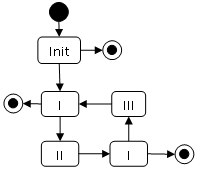
\includegraphics{sortingAlgorithm}
	\caption{Sorting algorithm}
	\label{fig:planning}
\end{figure}

Loop is going I, II, I, III, I... while do not get efficiency greater than 87\% (like set in configuration). By default if there are no configurations set, then algorithm works like presented in above chapter (sorting by color and temperature).

\begin{table}[h]
	
    \begin{tabular}{ | p{0.4cm} | p{1cm} | p{2cm} | p{1.7cm} |p{2cm} |p{1cm} |p{1.3cm} |p{1.2cm} |p{1.3cm} |}
    \hline
	Bin Id & Color & Washing Temperature & TotalBin Utilization (TBU) & NumberOf Bins Require (NBR) & Rest & Efficiency & Reserve & Success\\ \hline
	1 & White & 95 & 448\% & 4 & 48\% & 48\% & 52 \% & Fail \\ \hline
	2 & White & 60 & 818\% & 8 & 18\% & 18\% & 82 \% & Fail \\ \hline
	3 & White & 40 & 89\% & 1 & 0\% & 89\% & 11 \% & Pass \\ \hline
	4 & White & 30 & 639\% & 6 & 39\% & 39\% & 61 \% & Fail \\ \hline
	5 & White & HW & 159\% & - & - & - & - & - \\ \hline
	6 & Colored & 95 & 698\% & 7 & 0\% & 99\% & 2 \% & Pass \\ \hline
	7 & Colored & 60 & 2110\% & 21 & 10\% & 10\% & 90 \% & Fail \\ \hline
	8 & Colored & 40 & 788\% & 8 & 0\% & 98.5\% & 1.5 \% & Pass \\ \hline
	9 & Colored & 30 & 818\% & 9 & 0\% & 90.8\% & 9.2 \% & Pass \\ \hline
	10 & Colored & HW & 420\% & - & - & - & - & - \\ \hline
	11 & ... & ... & ... & ... & ... & ... & ... & ... \\ \hline
	- & - & - & - & - & - & Total: 62.54\% & - & All: No \\ \hline
    \end{tabular}
	\caption{Example of current state (when: Total washing machine value 87 \%)}
	\label{tab:AdDis}
\end{table}

Current state of the sorting is respresented by table where all values mutate during sort. Quantity of incomming clothes set bin ids and total bin utilization (TBU). TBU – how many times need to be washed it calculated by 8.1 formula:

Where clothe type can be: Sweater, Shirt, Pants, Underwear, WashingBag, Dress, Shorts, Towel and BedLinen. 



Efficiency can be calculated considering rest, diagram shown in figure 8.4. Efficiency describes is there cost-efficiency to wash or not. Wash is cost efficient than efficiency is greater 87\%.


\begin{figure}[h]
	\centering
		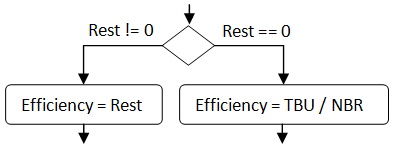
\includegraphics{efficiencyCalculation}
	\caption{Efficiency calculation diagram}
	\label{fig:planning}
\end{figure}

At the beginning incoming clothes are toke one after another and moved to the particular bin. If there are no clothes left than check how many distinct bins require. If there are more than zero bins than calculated and set current state like shown in the 8.1 table. If there are no clothes therefore there are no bins and algorithm is ended.

\begin{figure}[h]
	\centering
		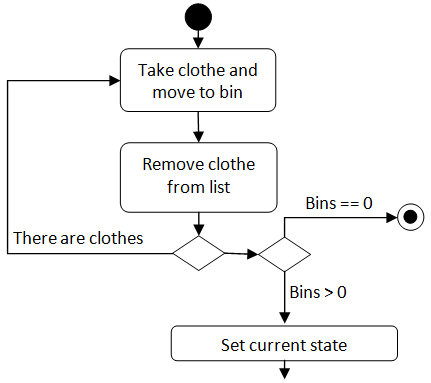
\includegraphics{diagramInit}
	\caption{Diagram Init}
	\label{fig:planning}
\end{figure}


Second move of algorithm is check for success and for time-out, figure 8.6. If all bins are greater efficiency than 87\% than current state is satisfied and clothes can be washed. In other case there is time-out algorithm also stopped. Purpose of the time-out added to avoid infinitive loop.

\begin{figure}[h]
	\centering
		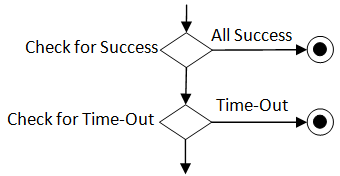
\includegraphics{diagramI}
	\caption{Diagram I}
	\label{fig:planning}
\end{figure}

Last two moves are very similar. Both of them try something to change when estimate current state and compare with previous. If new state is better than previous then state is set to current, in other case keep the last state. 

\begin{figure}[h]
	\centering
		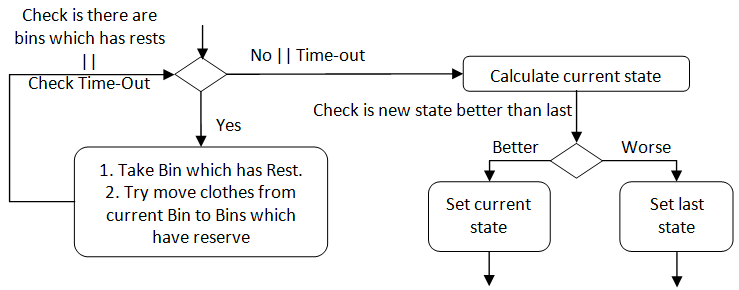
\includegraphics{diagramII}
	\caption{Diagram II}
	\label{fig:planning}
\end{figure}

At the figure 8.6 sorting algorithm trying to change the current state by moving clothes from bins which have rests to bins which have reserves and if result is better then new state set to current. 

\begin{figure}[h]
	\centering
		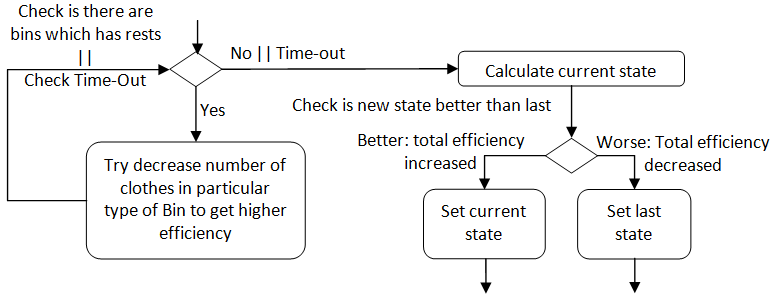
\includegraphics{diagramIII}
	\caption{Diagram III}
	\label{fig:planning}
\end{figure}

At the figure 8.7 sorting algorithm trying to change number of clothes in particular type of bin. For instance quantity of 818\% gives result for 8 bins and 18\% rest. However efficiency of 8 bins is 100\% and for the last one is only 18\%. Eight bins can be washed however the rest should be wait. So if there will be decreased number of clothes during one wash then could be increased efficiency. If 818\% of clothes we wash by 9 bins then we get efficiency of 90.8\% and reserve 9.2\%. So this is optimal and new state is set.

As we can see there are concurrency between II and III. If something changed at II then III have also possibilities to change and vice versa. Concurrency is essential to get a progress and mutation of states.